\documentclass{article}
\usepackage{amsmath}
\usepackage{amsfonts}
\usepackage{amssymb}
\usepackage{mathrsfs}
\usepackage{cancel}

\usepackage{graphicx}


\setlength\parindent{0pt}

\author{Pranav Tikkawar}
\title{Assignment 1: Stats 212}

\begin{document}
\maketitle
\section*{Problem 1}
\begin{figure}[h]
    \centering
    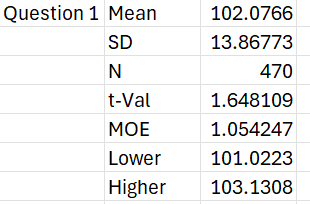
\includegraphics[width=0.5\textwidth]{A1img/Q1.png}
    \caption{Problem 1}
    \label{fig:Q1}
\end{figure}
Thus the 90\% confidence interval for the DVRT is $[101.0223, 103.13018]$.

\section*{Problem 2}
The interval we obtained, [101.0223, 103.13018], represents a range of values within which we are 90\% confident that the true value of the DVRT (whatever that may be) lies. This means that if we were to repeat the experiment multiple times and calculate the confidence interval each time, about 90\% of those intervals would contain the true value of the DVRT.

In simpler terms, it's like saying we are pretty sure that the DVRT value falls somewhere between 101.0223 and 103.13018, but we can't say with absolute certainty exactly what the true value is. The interval gives us a sense of the range of possible values.
\section*{Problem 3}
\begin{figure}[h]
    \centering
    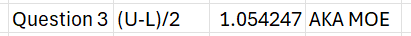
\includegraphics[width=0.5\textwidth]{A1img/Q3.png}
    \caption{Problem 3}
    \label{fig:Q1}
\end{figure}
The precision is determined by the upper and lower bounds of the confidence interval divided by two. In this case, the precision is $\frac{103.13018 - 101.0223}{2} = 1.05344$. It also is the Margin of Error.

\section*{Problem 4}

\begin{figure}[h]
    \centering
    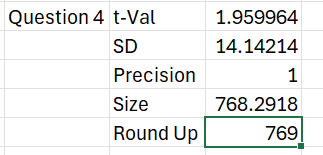
\includegraphics[width=0.5\textwidth]{A1img/Q4.png}
    \caption{Problem 1}
    \label{fig:Q3}
\end{figure}
The required sample size is 769 to estimate the precision of 1 unit with 95\% confidence.


\end{document}